\apendice{Especificación de Requisitos}

\section{Introducción}

En este anexo se recogen los objetivos del proyecto y los requisitos que definen el comportamiento del programa.

\section{Objetivos generales}

Con este proyecto se persigue la realización de los siguientes objetivos:

\begin{itemize}
    \item La instalación y configuración de un sistema capaz de recoger, almacenar y gestionar datos de sensores.
    \item La implementación de un motor de búsqueda para facilitar encontrar los datos deseados con la mayor precisión posible.
    \item Que la monitorización de los datos se muestre lo más clara y accesible posible para el usuario.
    \item Realizar un algoritmo de aprendizaje automático que pueda predecir comportamientos y patrones en los datos de los sensores.
\end{itemize}

\newpage
\section{Catálogo de requisitos}
A continuación, se procederá a enumerar los distintos requisitos funcionales:


\begin{itemize}

    \item \textbf{RF-1 Activar sistema}: El usuario ha de poder activar el sistema cuando desee.
    
    \item \textbf{RF-2 Desactivar sistema}: El usuario ha de poder desactivar el sistema cuando desee.
    
    \item \textbf{RF-3 Captación de sensores}: El sistema ha de almacenar los datos procedentes de los sensores.
    	
    \item \textbf{RF-4 Entrenamiento}: El sistema ha de entrenar un modelo con los datos de los sensores.

    \item \textbf{RF-5 Predicción}: El sistema ha de realizar una predicción sobre los datos de los sensores.

    \item \textbf{RF-6 Gestión del sistema}: El usuario ha de ser capaz de gestionar el sistema.
    \begin{itemize}
	    \item \textbf{RF-6.1 Añadir sensor}: El usuario ha de poder añadir sensores.
	    \item \textbf{RF-6.2 Borrar sensor}: El usuario ha de poder eliminar sensores.
	    \item \textbf{RF-6.3 Configurar modelo}: El usuario ha de poder configurar sus propios modelos.
	\end{itemize}
	
	\item \textbf{RF-7 Monitorización de datos}: El usuario ha de poder ver los datos de los sensores.
	\begin{itemize}
	    \item \textbf{RF-7.1 ver datos reales}: Se ha de monitorizar los datos reales procedentes del sensor.
	    \item \textbf{RF-7.2 ver datos entrenamiento}: Se ha de monitorizar los datos de entrenamiento del modelo.
	    \item \textbf{RF-7.3 ver datos predicción}: Se ha de monitorizar los datos de predicción.
	\end{itemize}
	\item \textbf{RF-8 Búsquedas filtradas}: El usuario ha de ser capaz de hacer búsquedas y filtrados de los datos.
	\item \textbf{RF-9 Representación gráfica}: El usuario ha de poder representar de forma gráfica los datos.
	\begin{itemize}
	    \item \textbf{RF-9.1 Creación de gráficas}: El usuario ha de poder crear gráficas.
	    \item \textbf{RF-9.2 Borrado de gráficas}: El usuario ha de poder borrar gráficas.
	    \item \textbf{RF-9.3 Visualización de gráficas}: El usuario ha de poder visualizar y consultar las gráficas creadas.
	\end{itemize}
	
\end{itemize}	
\newpage



\section{Especificación de requisitos}

En esta sección se mostrarán los casos de uso y su diagrama.

\subsection{Diagrama de casos de uso}

\begin{figure}[!h]
	\centering
	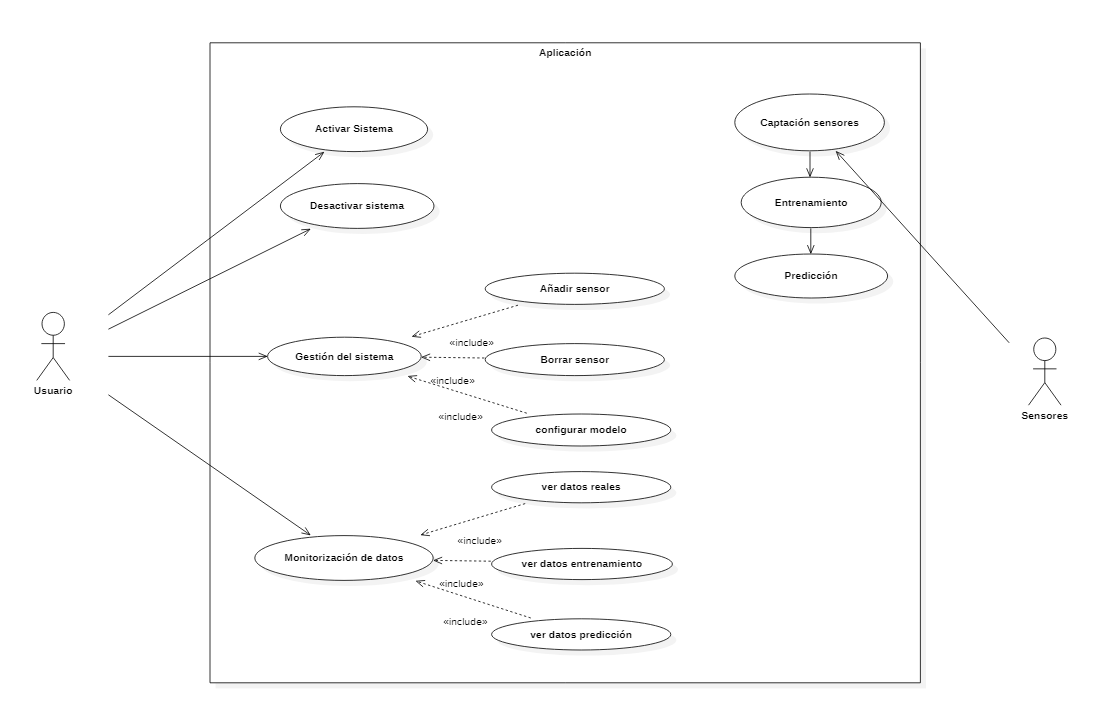
\includegraphics[width=1.2\textwidth]{img/img_casos_usos.png}
	\caption{Diagrama de casos de uso}
	\label{img_casos_usos}
\end{figure}
\clearpage

\subsection{Actores}
En esta aplicación interactúan dos actores, los sensores de los que se captan la información y el usuario que gestiona la aplicación y monitoriza el sistema.

\subsection{Casos de uso}
%Caso de uso 1
\tablaSmallSinColores{Caso de uso 1: Activar sistema.}{p{3cm} p{.75cm} p{9.5cm}}{tablaUC0}{
  \multicolumn{3}{l}{Caso de uso 1: Activar sistema.} \\
 }
 {
  Versión                            & \multicolumn{2}{p{10.25cm}}{1.0} \\\hline
  Autor                            & \multicolumn{2}{p{10.25cm}}{Daniel Mellado Hurtado} \\\hline
  Descripción                            & \multicolumn{2}{p{10.25cm}}{El usuario ha de poder activar el sistema cuando desee.} \\\hline
  \multirow{2}{3.5cm}{Requisitos}   &\multicolumn{2}{p{10.25cm}}{RF-1} \\\cline{2-3}

                                         \\\hline
                                         
  Precondiciones                         &  \multicolumn{2}{p{10.25cm}}{El programa ha de estar correctamente instalado.}   \\\hline
  \multirow{2}{3.5cm}{Secuencia normal}  & Paso & Acción \\\cline{2-3}
                                         & 1    & El usuario introduce el comando de inicialización del programa en la consola
  

                                         \\\hline
  Postcondiciones                        & \multicolumn{2}{p{10.25cm}}{El sistema se encuentra activo y funcionando} \\\hline
  Excepciones                        & \multicolumn{2}{p{10.25cm}}{No se encuentra el servicio correspondiente al programa.}\\\hline
  Importancia                            & Alta \\\hline
  Urgencia                               & Alta \\
}

%Caso de uso 2
\tablaSmallSinColores{Caso de uso 2: Desactivar sistema.}{p{3cm} p{.75cm} p{9.5cm}}{tablaUC0}{
  \multicolumn{3}{l}{Caso de uso 2: Desactivar sistema.} \\
 }
 {
  Versión                            & \multicolumn{2}{p{10.25cm}}{1.0} \\\hline
  Autor                            & \multicolumn{2}{p{10.25cm}}{Daniel Mellado Hurtado} \\\hline
  Descripción                            & \multicolumn{2}{p{10.25cm}}{El usuario ha de poder desactivar el sistema cuando desee.} \\\hline
  \multirow{2}{3.5cm}{Requisitos}   &\multicolumn{2}{p{10.25cm}}{RF-2} \\\cline{2-3}

                                         \\\hline
                                         
  Precondiciones                         &  \multicolumn{2}{p{10.25cm}}{El sistema se encuentra activo}   \\\hline
  \multirow{2}{3.5cm}{Secuencia normal}  & Paso & Acción \\\cline{2-3}
                                         & 1    & El usuario introduce el comando de parada del programa en la consola


                                         \\\hline
  Postcondiciones                        & \multicolumn{2}{p{10.25cm}}{El sistema se encuentra desactivado} \\\hline
  Excepciones                        & \multicolumn{2}{p{10.25cm}}{}\\\hline
  Importancia                            & Alta \\\hline
  Urgencia                               & Alta \\
}

%Caso de uso 3
\tablaSmallSinColores{Caso de uso 3: Almacenamiento de datos.}{p{3cm} p{.75cm} p{9.5cm}}{tablaUC0}{
  \multicolumn{3}{l}{Caso de uso 3: Almacenamiento de datos.} \\
 }
 {
  Versión                            & \multicolumn{2}{p{10.25cm}}{1.0} \\\hline
  Autor                            & \multicolumn{2}{p{10.25cm}}{Daniel Mellado Hurtado} \\\hline
  Descripción                            & \multicolumn{2}{p{10.25cm}}{El sistema ha de almacenar los datos procedentes de los sensores} \\\hline
  \multirow{2}{3.5cm}{Requisitos}   &\multicolumn{2}{p{10.25cm}}{RF-3} \\\cline{2-3}

                                         \\\hline
                                         
  Precondiciones                         &  \multicolumn{2}{p{10.25cm}}{Los sensores se encuentran activos y PRTG recibe sus datos}   \\\hline
  \multirow{2}{3.5cm}{Secuencia normal}  & Paso & Acción \\\cline{2-3}
                                         & 1    & El sistema descarga los datos procedentes de PRTG
  \\\cline{2-3}
                                         & 2    & Se transforman los datos descargados
    \\\cline{2-3}
                                         & 3    & El sistema envía los datos a Elasicsearch 
                                         \\\hline
  Postcondiciones                        & \multicolumn{2}{p{10.25cm}}{Los datos de los sensores son recogidos y almacenados correctamente} \\\hline
  Excepciones                        & \multicolumn{2}{p{10.25cm}}{No se encuentra el servidor de PRTG. No hay datos disponibles}\\\hline
  Importancia                            & Alta \\\hline
  Urgencia                               & Alta \\
}

%Caso de uso 4
\tablaSmallSinColores{Caso de uso 4: Entrenamiento.}{p{3cm} p{.75cm} p{9.5cm}}{tablaUC0}{
  \multicolumn{3}{l}{Caso de uso 4: Entrenamiento.} \\
 }
 {
  Versión                            & \multicolumn{2}{p{10.25cm}}{1.0} \\\hline
  Autor                            & \multicolumn{2}{p{10.25cm}}{Daniel Mellado Hurtado} \\\hline
  Descripción                            & \multicolumn{2}{p{10.25cm}}{El sistema ha de entrenar un modelo con los datos de los sensores} \\\hline
  \multirow{2}{3.5cm}{Requisitos}   &\multicolumn{2}{p{10.25cm}}{RF-4} \\\cline{2-3}
                                         & \multicolumn{2}{p{10.25cm}}{}
                                         \\\hline
                                         
  Precondiciones                         &  \multicolumn{2}{p{10.25cm}}{Existen datos de los sensores en Elasitcsearch. Exista un modelo para cada sensor que se vaya a entrenar}   \\\hline
  \multirow{2}{3.5cm}{Secuencia normal}  & Paso & Acción \\\cline{2-3}
                                         & 1    & El sistema descarga los datos que se desea entrenar de Elasticsearch
  \\\cline{2-3}
                                         & 2    & Se carga el modelo asociado a dicho sensor
  \\\cline{2-3}
                                         & 3    & Se realiza el entrenamiento.
    \\\cline{2-3}
                                         & 4    & Se suben los datos del entrenamiento
    \\\cline{2-3}
                                         & 5    & Se guarda el modelo entrenado.
                                         \\\hline
  Postcondiciones                        & \multicolumn{2}{p{10.25cm}}{El modelo se encuentra entrenado.} \\\hline
  Excepciones                        & \multicolumn{2}{p{10.25cm}}{No existen datos en Elasticsearch para dicho sensor. No se encuentra un modelo para dicho sensor}\\\hline
  Importancia                            & Media \\\hline
  Urgencia                               & Media \\
}

%Caso de uso 5
\tablaSmallSinColores{Caso de uso 5: Predicción.}{p{3cm} p{.75cm} p{9.5cm}}{tablaUC0}{
  \multicolumn{3}{l}{Caso de uso 5: Predicción.} \\
 }
 {
  Versión                            & \multicolumn{2}{p{10.25cm}}{1.0} \\\hline
  Autor                            & \multicolumn{2}{p{10.25cm}}{Daniel Mellado Hurtado} \\\hline
  Descripción                            & \multicolumn{2}{p{10.25cm}}{El sistema ha de realizar una predicción sobre los datos de los sensores.} \\\hline
  \multirow{2}{3.5cm}{Requisitos}   &\multicolumn{2}{p{10.25cm}}{RF-5} \\\cline{2-3}
                                         & \multicolumn{2}{p{10.25cm}}{}
                                         \\\hline
                                         
  Precondiciones                         &  \multicolumn{2}{p{10.25cm}}{Exista un modelo para cada sensor que se vaya a predecir}   \\\hline
  \multirow{2}{3.5cm}{Secuencia normal}  & Paso & Acción \\\cline{2-3}
                                         & 1    & El sistema carga el modelo del sensor que se vaya a predecir
  \\\cline{2-3}
                                         & 2    & Se realiza la predicción
  \\\cline{2-3}
                                         & 3    & Se suben los datos de la predicción a Elasticsearch
.
                                         \\\hline
  Postcondiciones                        & \multicolumn{2}{p{10.25cm}}{Se ha realizado la predicción de un sensor} \\\hline
  Excepciones                        & \multicolumn{2}{p{10.25cm}}{No se encuentra un modelo para dicho sensor}\\\hline
  Importancia                            & Media \\\hline
  Urgencia                               & Media \\
}



%Caso de uso 6
\tablaSmallSinColores{Caso de uso 6: Gestión del sistema.}{p{3cm} p{.75cm} p{9.5cm}}{tablaUC0}{
  \multicolumn{3}{l}{Caso de uso 6: Gestión del sistema.} \\
 }
 {
  Versión                            & \multicolumn{2}{p{10.25cm}}{1.0} \\\hline
  Autor                            & \multicolumn{2}{p{10.25cm}}{Daniel Mellado Hurtado} \\\hline
  Descripción                            & \multicolumn{2}{p{10.25cm}}{El usuario ha de ser capaz de gestionar el sistema.} \\\hline
  \multirow{2}{3.5cm}{Requisitos}   &\multicolumn{2}{p{10.25cm}}{RF-6} \\\cline{2-3}
                                         & \multicolumn{2}{p{10.25cm}}{RF-6.1, RF-6.2, RF-6.3}
                                         \\\hline
                                         
  Precondiciones                         &  \multicolumn{2}{p{10.25cm}}{El sistema se encuentra funcionando. El usuario posee permisos de administrador.}   \\\hline
  \multirow{2}{3.5cm}{Secuencia normal}  & Paso & Acción \\\cline{2-3}
                                         & 1    & El usuario entra al fichero de configuración.
  \\\cline{2-3}
                                         & 2    & Se muestran las variables que se pueden configurar.
  \\\cline{2-3}
                                         & 3    & El usuario guarda el fichero.
   \\\cline{2-3}
                                         & 4    & El usuario reinicia el programa.
                                         \\\hline
  Postcondiciones                        & \multicolumn{2}{p{10.25cm}}{El sistema se encuentra configurado.} \\\hline
  Excepciones                        & \multicolumn{2}{p{10.25cm}}{Algún dato introducido es inválido.}\\\hline
  Importancia                            & Alta \\\hline
  Urgencia                               & Alta \\
}

%Caso de uso 7
\tablaSmallSinColores{Caso de uso 7: Añadir sensor.}{p{3cm} p{.75cm} p{9.5cm}}{tablaUC0}{
  \multicolumn{3}{l}{Caso de uso 7: Añadir sensor.} \\
 }
 {
  Versión                            & \multicolumn{2}{p{10.25cm}}{1.0} \\\hline
  Autor                            & \multicolumn{2}{p{10.25cm}}{Daniel Mellado Hurtado} \\\hline
  Descripción                            & \multicolumn{2}{p{10.25cm}}{El usuario ha de poder añadir sensores.} \\\hline
  \multirow{2}{3.5cm}{Requisitos}   &\multicolumn{2}{p{10.25cm}}{RF-6.1} \\\cline{2-3}
                                         & \multicolumn{2}{p{10.25cm}}{}
                                         \\\hline
                                         
  Precondiciones                         &  \multicolumn{2}{p{10.25cm}}{El sistema se encuentra funcionando.}   \\\hline
  \multirow{2}{3.5cm}{Secuencia normal}  & Paso & Acción \\\cline{2-3}
                                         & 1    & El usuario entra al fichero de configuración.
  \\\cline{2-3}
                                         & 2    & Se muestra la lista de ids de sensores.
  \\\cline{2-3}
                                         & 3    & El usuario añade uno o varios sensores.
     \\\cline{2-3}
                                         & 3    & El usuario guarda el fichero. 
   \\\cline{2-3}
                                         & 4    & El usuario reinicia el programa.                                       
.
                                         \\\hline
  Postcondiciones                        & \multicolumn{2}{p{10.25cm}}{El programa realizara la obtención, entrenamiento y predicción de los nuevos sensores introducidos.} \\\hline
  Excepciones                        & \multicolumn{2}{p{10.25cm}}{No se encuentran los sensores introducidos}\\\hline
  Importancia                            & Alta \\\hline
  Urgencia                               & Alta \\
}

%Caso de uso 8
\tablaSmallSinColores{Caso de uso 8: Borrar sensor}{p{3cm} p{.75cm} p{9.5cm}}{tablaUC0}{
  \multicolumn{3}{l}{Caso de uso 8: Borrar sensor.} \\
 }
 {
  Versión                            & \multicolumn{2}{p{10.25cm}}{1.0} \\\hline
  Autor                            & \multicolumn{2}{p{10.25cm}}{Daniel Mellado Hurtado} \\\hline
  Descripción                            & \multicolumn{2}{p{10.25cm}}{El usuario ha de poder eliminar sensores.} \\\hline
  \multirow{2}{3.5cm}{Requisitos}   &\multicolumn{2}{p{10.25cm}}{RF-6.2} \\\cline{2-3}
                                         & \multicolumn{2}{p{10.25cm}}{}
                                         \\\hline
                                         
  Precondiciones                         &  \multicolumn{2}{p{10.25cm}}{El sistema se encuentra funcionando.}   \\\hline
  \multirow{2}{3.5cm}{Secuencia normal}  & Paso & Acción \\\cline{2-3}
                                         & 1    & El usuario entra al fichero de configuración.
  \\\cline{2-3}
                                         & 2    & Se muestra la lista de ids de sensores.
  \\\cline{2-3}
                                         & 3    & El usuario elimina uno o varios sensores.
     \\\cline{2-3}
                                         & 3    & El usuario guarda el fichero. 
   \\\cline{2-3}
                                         & 4    & El usuario reinicia el programa.                                       
.
                                         \\\hline
  Postcondiciones                        & \multicolumn{2}{p{10.25cm}}{El programa ya no realizara la obtención, entrenamiento y predicción de los nuevos sensores eliminados.} \\\hline
  Excepciones                        & \multicolumn{2}{p{10.25cm}}{}\\\hline
  Importancia                            & Alta \\\hline
  Urgencia                               & Alta \\
}

%Caso de uso 9
\tablaSmallSinColores{Caso de uso 9: Configurar modelo.}{p{3cm} p{.75cm} p{9.5cm}}{tablaUC0}{
  \multicolumn{3}{l}{Caso de uso 9: Configurar modelo.} \\
 }
 {
  Versión                            & \multicolumn{2}{p{10.25cm}}{1.0} \\\hline
  Autor                            & \multicolumn{2}{p{10.25cm}}{Daniel Mellado Hurtado} \\\hline
  Descripción                            & \multicolumn{2}{p{10.25cm}}{El usuario ha de poder configurar sus propios modelos.} \\\hline
  \multirow{2}{3.5cm}{Requisitos}   &\multicolumn{2}{p{10.25cm}}{RF-6.3} \\\cline{2-3}
                                         & \multicolumn{2}{p{10.25cm}}{}
                                         \\\hline
                                         
  Precondiciones                         &  \multicolumn{2}{p{10.25cm}}{El sistema se encuentra funcionando.}   \\\hline
  \multirow{2}{3.5cm}{Secuencia normal}  & Paso & Acción \\\cline{2-3}
                                         & 1    & El usuario entra al fichero de Crear modelo.
  \\\cline{2-3}
                                         & 2    & El usuario especifica el id del sensor con el cual se va a entrenar el modelo.
  \\\cline{2-3}
                                         & 3    & El usuario elige el tipo de modelo de desea utilizar
     \\\cline{2-3}
                                         & 3    & El usuario introduce los parámetros de dicho modelo
   \\\cline{2-3}
                                         & 4    & El usuario ejecuta el fichero de crear modelo         
                                         
    \\\cline{2-3}
                                         & 5    & El sistema guarda el nuevo modelo en disco.
.
                                         \\\hline
  Postcondiciones                        & \multicolumn{2}{p{10.25cm}}{El modelo se encuentra guardado y podrá ser utilizado para el entrenamiento y la predicción} \\\hline
  Excepciones                        & \multicolumn{2}{p{10.25cm}}{El modelo que se desea implementar no existe.}\\\hline
  Importancia                            & Alta \\\hline
  Urgencia                               & Alta \\
}

%Caso de uso 10
\tablaSmallSinColores{Caso de uso 10: Monitorización de datos.}{p{3cm} p{.75cm} p{9.5cm}}{tablaUC0}{
  \multicolumn{3}{l}{Caso de uso 10: Monitorización de datos.} \\
 }
 {
  Versión                            & \multicolumn{2}{p{10.25cm}}{1.0} \\\hline
  Autor                            & \multicolumn{2}{p{10.25cm}}{Daniel Mellado Hurtado} \\\hline
  Descripción                            & \multicolumn{2}{p{10.25cm}}{El usuario ha de poder ver los datos de los sensores.} \\\hline
  \multirow{2}{3.5cm}{Requisitos}   &\multicolumn{2}{p{10.25cm}}{RF-7} \\\cline{2-3}
                                         & \multicolumn{2}{p{10.25cm}}{RF-7.1, RF-7.2, RF-7.3}
                                         \\\hline
                                         
  Precondiciones                         &  \multicolumn{2}{p{10.25cm}}{El sistema se encuentra funcionando.}   \\\hline
  \multirow{2}{3.5cm}{Secuencia normal}  & Paso & Acción \\\cline{2-3}
                                         & 1    & El usuario accede a la url de Kibana.
  \\\cline{2-3}
                                         & 2    & El usuario accede al apartado \textit{Discover}.
  \\\cline{2-3}
                                         & 3    & El usuario elige un rango de fechas
  \\\cline{2-3}
                                         & 4   & El usuario introduce filtra los datos por los campos que vea apropiados.
        
                                         \\\hline
  Postcondiciones                        & \multicolumn{2}{p{10.25cm}}{Se muestran los datos de los sensores} \\\hline
  Excepciones                        & \multicolumn{2}{p{10.25cm}}{No existen datos.}\\\hline
  Importancia                            & Alta \\\hline
  Urgencia                               & Alta \\
}

%Caso de uso 11
\tablaSmallSinColores{Caso de uso 11: Ver datos reales.}{p{3cm} p{.75cm} p{9.5cm}}{tablaUC0}{
  \multicolumn{3}{l}{Caso de uso 11: Ver datos reales.} \\
 }
 {
  Versión                            & \multicolumn{2}{p{10.25cm}}{1.0} \\\hline
  Autor                            & \multicolumn{2}{p{10.25cm}}{Daniel Mellado Hurtado} \\\hline
  Descripción                            & \multicolumn{2}{p{10.25cm}}{Se ha de monitorizar los datos reales procedentes del sensor.} \\\hline
  \multirow{2}{3.5cm}{Requisitos}   &\multicolumn{2}{p{10.25cm}}{RF-7.1} \\\cline{2-3}
                                         & \multicolumn{2}{p{10.25cm}}{}
                                         \\\hline
                                         
  Precondiciones                         &  \multicolumn{2}{p{10.25cm}}{El sistema se encuentra funcionando.}   \\\hline
  \multirow{2}{3.5cm}{Secuencia normal}  & Paso & Acción \\\cline{2-3}
                                         & 1    & El usuario accede a la url de Kibana.
  \\\cline{2-3}
                                         & 2    & El usuario accede al apartado \textit{Discover}.
  \\\cline{2-3}
                                         & 3    & El usuario elige un rango de fechas
  \\\cline{2-3}
                                         & 4    & El usuario introduce filtra por el campo \textit{valor}
        
                                         \\\hline
  Postcondiciones                        & \multicolumn{2}{p{10.25cm}}{Se muestran los valores reales de los sensores} \\\hline
  Excepciones                        & \multicolumn{2}{p{10.25cm}}{No existen datos.}\\\hline
  Importancia                            & Alta \\\hline
  Urgencia                               & Alta \\
}

%Caso de uso 12
\tablaSmallSinColores{Caso de uso 12: Ver datos entrenamiento.}{p{3cm} p{.75cm} p{9.5cm}}{tablaUC0}{
  \multicolumn{3}{l}{Caso de uso 12: Ver datos entrenamiento.} \\
 }
 {
  Versión                            & \multicolumn{2}{p{10.25cm}}{1.0} \\\hline
  Autor                            & \multicolumn{2}{p{10.25cm}}{Daniel Mellado Hurtado} \\\hline
  Descripción                            & \multicolumn{2}{p{10.25cm}}{Se ha de monitorizar los datos de entrenamiento procedentes del sensor.} \\\hline
  \multirow{2}{3.5cm}{Requisitos}   &\multicolumn{2}{p{10.25cm}}{RF-7.2} \\\cline{2-3}
                                         & \multicolumn{2}{p{10.25cm}}{}
                                         \\\hline
                                         
  Precondiciones                         &  \multicolumn{2}{p{10.25cm}}{El sistema se encuentra funcionando.}   \\\hline
  \multirow{2}{3.5cm}{Secuencia normal}  & Paso & Acción \\\cline{2-3}
                                         & 1    & El usuario accede a la url de Kibana.
  \\\cline{2-3}
                                         & 2    & El usuario accede al apartado \textit{Discover}.
  \\\cline{2-3}
                                         & 3    & El usuario elige un rango de fechas
  \\\cline{2-3}
                                         & 4    & El usuario introduce filtra por el campo \textit{entrenamiento}
        
                                         \\\hline
  Postcondiciones                        & \multicolumn{2}{p{10.25cm}}{Se muestran los valores de entrenamiento de los sensores} \\\hline
  Excepciones                        & \multicolumn{2}{p{10.25cm}}{No existen datos.}\\\hline
  Importancia                            & Alta \\\hline
  Urgencia                               & Alta \\
}

%Caso de uso 12
\tablaSmallSinColores{Caso de uso 12: Ver datos predicción.}{p{3cm} p{.75cm} p{9.5cm}}{tablaUC0}{
  \multicolumn{3}{l}{Caso de uso 12: Ver datos predicción.} \\
 }
 {
  Versión                            & \multicolumn{2}{p{10.25cm}}{1.0} \\\hline
  Autor                            & \multicolumn{2}{p{10.25cm}}{Daniel Mellado Hurtado} \\\hline
  Descripción                            & \multicolumn{2}{p{10.25cm}}{Se ha de monitorizar los datos de predicción del sensor.} \\\hline
  \multirow{2}{3.5cm}{Requisitos}   &\multicolumn{2}{p{10.25cm}}{RF-7.3} \\\cline{2-3}
                                         & \multicolumn{2}{p{10.25cm}}{}
                                         \\\hline
                                         
  Precondiciones                         &  \multicolumn{2}{p{10.25cm}}{El sistema se encuentra funcionando.}   \\\hline
  \multirow{2}{3.5cm}{Secuencia normal}  & Paso & Acción \\\cline{2-3}
                                         & 1    & El usuario accede a la url de Kibana.
  \\\cline{2-3}
                                         & 2    & El usuario accede al apartado \textit{Discover}.
  \\\cline{2-3}
                                         & 3    & El usuario elige un rango de fechas
  \\\cline{2-3}
                                         & 4    & El usuario introduce filtra por el campo \textit{prediccion}
        
                                         \\\hline
  Postcondiciones                        & \multicolumn{2}{p{10.25cm}}{Se muestran los valores de predicción de los sensores} \\\hline
  Excepciones                        & \multicolumn{2}{p{10.25cm}}{Elasticsearch no está activo, Kibana no esta activo.}\\\hline
  Importancia                            & Alta \\\hline
  Urgencia                               & Alta \\
}


%Caso de uso 13
\tablaSmallSinColores{Caso de uso 13: Búsquedas filtradas.}{p{3cm} p{.75cm} p{9.5cm}}{tablaUC0}{
  \multicolumn{3}{l}{Caso de uso 13: Búsquedas filtradas.} \\
 }
 {
  Versión                            & \multicolumn{2}{p{10.25cm}}{1.0} \\\hline
  Autor                            & \multicolumn{2}{p{10.25cm}}{Daniel Mellado Hurtado} \\\hline
  Descripción                            & \multicolumn{2}{p{10.25cm}}{El usuario ha de ser capaz de hacer búsquedas y filtrados de los datos.} \\\hline
  \multirow{2}{3.5cm}{Requisitos}   &\multicolumn{2}{p{10.25cm}}{RF-8} \\\cline{2-3}
                                         & \multicolumn{2}{p{10.25cm}}{}
                                         \\\hline
                                         
  Precondiciones                         &  \multicolumn{2}{p{10.25cm}}{Elasticsearch y Kibana se encuentran funcionando}   \\\hline
  \multirow{2}{3.5cm}{Secuencia normal}  & Paso & Acción \\\cline{2-3}
                                         & 1    & El usuario accede a la url de Kibana.
  \\\cline{2-3}
                                         & 2    & El usuario accede al apartado \textit{Discover}.
  \\\cline{2-3}
                                         & 3    & El usuario elige un rango de fechas
  \\\cline{2-3}
                                         & 4    & El usuario introduce las restricciones que se desea en el buscador y en los filtros.
        
                                         \\\hline
  Postcondiciones                        & \multicolumn{2}{p{10.25cm}}{Se muestran los valores filtrados} \\\hline
  Excepciones                        & \multicolumn{2}{p{10.25cm}}{No existen datos.}\\\hline
  Importancia                            & Alta \\\hline
  Urgencia                               & Alta \\
}



%Caso de uso 14
\tablaSmallSinColores{Caso de uso 14: Representación gráfica.}{p{3cm} p{.75cm} p{9.5cm}}{tablaUC0}{
  \multicolumn{3}{l}{Caso de uso 14: Representación gráficas.} \\
 }
 {
  Versión                            & \multicolumn{2}{p{10.25cm}}{1.0} \\\hline
  Autor                            & \multicolumn{2}{p{10.25cm}}{Daniel Mellado Hurtado} \\\hline
  Descripción                            & \multicolumn{2}{p{10.25cm}}{El usuario ha de poder representar de forma gráfica los datos.} \\\hline
  \multirow{2}{3.5cm}{Requisitos}   &\multicolumn{2}{p{10.25cm}}{RF-9} \\\cline{2-3}
                                         & \multicolumn{2}{p{10.25cm}}{RF-9.1, RF-9.2, RF-9.3}
                                         \\\hline
                                         
  Precondiciones                         &  \multicolumn{2}{p{10.25cm}}{Elasticsearch y Kibana se encuentran funcionando}   \\\hline
  \multirow{2}{3.5cm}{Secuencia normal}  & Paso & Acción \\\cline{2-3}
                                         & 1    & El usuario accede a la url de Kibana.
  \\\cline{2-3}
                                         & 2    & El usuario accede al apartado \textit{Dashboards}.

                                         \\\hline
  Postcondiciones                        & \multicolumn{2}{p{10.25cm}}{} \\\hline
  Excepciones                        & \multicolumn{2}{p{10.25cm}}{No existen datos.}\\\hline
  Importancia                            & Alta \\\hline
  Urgencia                               & Alta \\
}


%Caso de uso 15
\tablaSmallSinColores{Caso de uso 15: Creación de gráficas.}{p{3cm} p{.75cm} p{9.5cm}}{tablaUC0}{
  \multicolumn{3}{l}{Caso de uso 15: Creación de gráficas.} \\
 }
 {
  Versión                            & \multicolumn{2}{p{10.25cm}}{1.0} \\\hline
  Autor                            & \multicolumn{2}{p{10.25cm}}{Daniel Mellado Hurtado} \\\hline
  Descripción                            & \multicolumn{2}{p{10.25cm}}{El usuario ha de poder crear gráficas.} \\\hline
  \multirow{2}{3.5cm}{Requisitos}   &\multicolumn{2}{p{10.25cm}}{RF-9.1} \\\cline{2-3}
                                         & \multicolumn{2}{p{10.25cm}}{}
                                         \\\hline
                                         
  Precondiciones                         &  \multicolumn{2}{p{10.25cm}}{Elasticsearch y Kibana se encuentran funcionando}   \\\hline
  \multirow{2}{3.5cm}{Secuencia normal}  & Paso & Acción \\\cline{2-3}
                                         & 1    & El usuario accede a la url de Kibana.
  \\\cline{2-3}
                                         & 2    & El usuario accede al apartado \textit{Dashboards}.
  \\\cline{2-3}
                                         & 3    & El usuario da al botón \textit{Create Dashboard}
  \\\cline{2-3}
                                         & 4    & El usuario da al botón \textit{Create Visualization}
  \\\cline{2-3}
                                         & 5    & El usuario elige el tipo de gráfico
  \\\cline{2-3}
                                         & 6    & El usuario introduce las variables que se van a representar.
    \\\cline{2-3}
                                         & 7    & El usuari guarda el grafico, dando al botón \textit{save and return}.
        
                                         \\\hline
  Postcondiciones                        & \multicolumn{2}{p{10.25cm}}{Se ha creado un gráfico representando las variables elegidas.} \\\hline
  Excepciones                        & \multicolumn{2}{p{10.25cm}}{No existen datos.}\\\hline
  Importancia                            & Alta \\\hline
  Urgencia                               & Alta \\
}

%Caso de uso 16
\tablaSmallSinColores{Caso de uso 16: Borrado de gráficas.}{p{3cm} p{.75cm} p{9.5cm}}{tablaUC0}{
  \multicolumn{3}{l}{Caso de uso 16: Borrado de gráficas.} \\
 }
 {
  Versión                            & \multicolumn{2}{p{10.25cm}}{1.0} \\\hline
  Autor                            & \multicolumn{2}{p{10.25cm}}{Daniel Mellado Hurtado} \\\hline
  Descripción                            & \multicolumn{2}{p{10.25cm}}{El usuario ha de poder borrar gráficas.} \\\hline
  \multirow{2}{3.5cm}{Requisitos}   &\multicolumn{2}{p{10.25cm}}{RF-9.2} \\\cline{2-3}
                                         & \multicolumn{2}{p{10.25cm}}{}
                                         \\\hline
                                         
  Precondiciones                         &  \multicolumn{2}{p{10.25cm}}{Elasticsearch y Kibana se encuentran funcionando}   \\\hline
  \multirow{2}{3.5cm}{Secuencia normal}  & Paso & Acción \\\cline{2-3}
                                         & 1    & El usuario accede a la url de Kibana.
  \\\cline{2-3}
                                         & 2    & El usuario accede al apartado \textit{Dashboards}.
  \\\cline{2-3}
                                         & 3    & El usuario accede al la ruleta de opciones del gráfico que se desea eliminar
  \\\cline{2-3}
                                         & 4    & El usuario selecciona la opción \textit{more}
  \\\cline{2-3}
                                         & 5    & El usuario selecciona la opción \textit{Delete from Dashboards}
.
        
                                         \\\hline
  Postcondiciones                        & \multicolumn{2}{p{10.25cm}}{La gráfica se borra} \\\hline
  Excepciones                        & \multicolumn{2}{p{10.25cm}}{}\\\hline
  Importancia                            & Alta \\\hline
  Urgencia                               & Alta \\
}

%Caso de uso 17
\tablaSmallSinColores{Caso de uso 16: Visualización de gráficas.}{p{3cm} p{.75cm} p{9.5cm}}{tablaUC0}{
  \multicolumn{3}{l}{Caso de uso 16:Visualización de gráficas.} \\
 }
 {
  Versión                            & \multicolumn{2}{p{10.25cm}}{1.0} \\\hline
  Autor                            & \multicolumn{2}{p{10.25cm}}{Daniel Mellado Hurtado} \\\hline
  Descripción                            & \multicolumn{2}{p{10.25cm}}{El usuario ha de poder visualizar y consultar las gráficas creadas} \\\hline
  \multirow{2}{3.5cm}{Requisitos}   &\multicolumn{2}{p{10.25cm}}{RF-9.3} \\\cline{2-3}
                                         & \multicolumn{2}{p{10.25cm}}{}
                                         \\\hline
                                         
  Precondiciones                         &  \multicolumn{2}{p{10.25cm}}{Elasticsearch y Kibana se encuentran funcionando}   \\\hline
  \multirow{2}{3.5cm}{Secuencia normal}  & Paso & Acción \\\cline{2-3}
                                         & 1    & El usuario accede a la url de Kibana.
  \\\cline{2-3}
                                         & 2    & El usuario accede al apartado \textit{Dashboards}.
  \\\cline{2-3}
                                         & 2    & El usuario elige el rango de fechas para ver los datos representados en las gráficas

                                         \\\hline
  Postcondiciones                        & \multicolumn{2}{p{10.25cm}}{Se muestran todas las gráficas creadas} \\\hline
  Excepciones                        & \multicolumn{2}{p{10.25cm}}{}\\\hline
  Importancia                            & Alta \\\hline
  Urgencia                               & Alta \\
}